\documentclass[x11names,svgnames,11pt]{beamer}

%\usepackage[orientation=landscape,size=a0,scale=1.26,debug]{beamerposter}    % beamer in poster size

\usetheme{sharky}

\usepackage[compatibility=false, justification=justified]{caption}    % to allow the use of \caption* i.e. caption without numbering

\usepackage{media9}

\usepackage{amssymb}
\usepackage[T1]{fontenc}

\usepackage{color}
\definecolor{mygreen}{rgb}{0,0.6,0}
\definecolor{mygray}{rgb}{0.90,0.90,0.90}
\definecolor{mymauve}{rgb}{0.58,0,0.82}
\definecolor{myblue}{rgb}{0.0, 0.18, 0.65}

%colors and fontsize of blocks
\usepackage{tcolorbox}
\tcbset{%
    noparskip,
    colback=mygray, %background color of the box
    colframe=sharky_main, %color of frame and title background
    coltext=black, %color of body text
    coltitle=black, %color of title text 
    fonttitle=\tiny\bfseries, %style and size of title font
    fontupper=\tiny, %style and size of text font
    boxsep=1pt,
     left=1pt,
     right=1pt,
     top=1pt,
     bottom=1pt
    }

\usepackage{listings} % for displaying programming code in LaTex (see: https://www.sharelatex.com/learn/Code_listing) 
 \lstset{basicstyle=\tiny\ttfamily,  % size and style of fonts used for the code
      backgroundcolor=\color{white},  % choose the background color
      breaklines=true,                          % break lines when too long 
      linewidth=0.9\linewidth,
      resetmargins=true,                      % reset the margins
      %xleftmargin=0.0cm,                 % set the left margin
      %xrightmargin=1.0cm,                   % set the right margin
      showspaces=false,                       % show spaces adding particular underscores
      showstringspaces=false,             % underline spaces within strings
      showtabs=false,                          % show tabs within strings adding 
      escapechar=@,                             % to add LaTeX commands within the code
      keywordstyle=\color{mygreen},  % keyword style
      commentstyle=\color{bluegray},   % comment style
      stringstyle=\color{red},       % string literal style
      language=Python,
      morekeywords={True,False}
} 

\usepackage{hyperref}
\hypersetup{
    colorlinks=true,
    linkcolor=blue,
    filecolor=blue,      
    urlcolor=blue,
}
\urlstyle{same}

\usepackage{changepage}
\usepackage{bold-extra}

\lstset{
escapeinside=| |
}

\begin{document} %start of the document

\begin{frame}[plain,fragile]%each beamer presentation is coded like a single slide called "Frame"
	
	\textbf{\color{myblue} Exploring complex systems using computational tools}\\
	Matplotlib Cheat Sheet\\
	
	\begin{columns}
		\column{0.6\linewidth}	
			\begin{tcolorbox}[title=Matplotlib]
		 		Matplotlib (matplotlib.org) is a Python 2D plotting library which produces publication
				 quality figures  in a variety of hardcopy formats and interactive environments across
				 platforms. 
			\end{tcolorbox}
		
			\begin{tcolorbox}[title=Workflow]
				\begin{columns}
					\column{0.025\linewidth}
					\column{0.45\linewidth}
						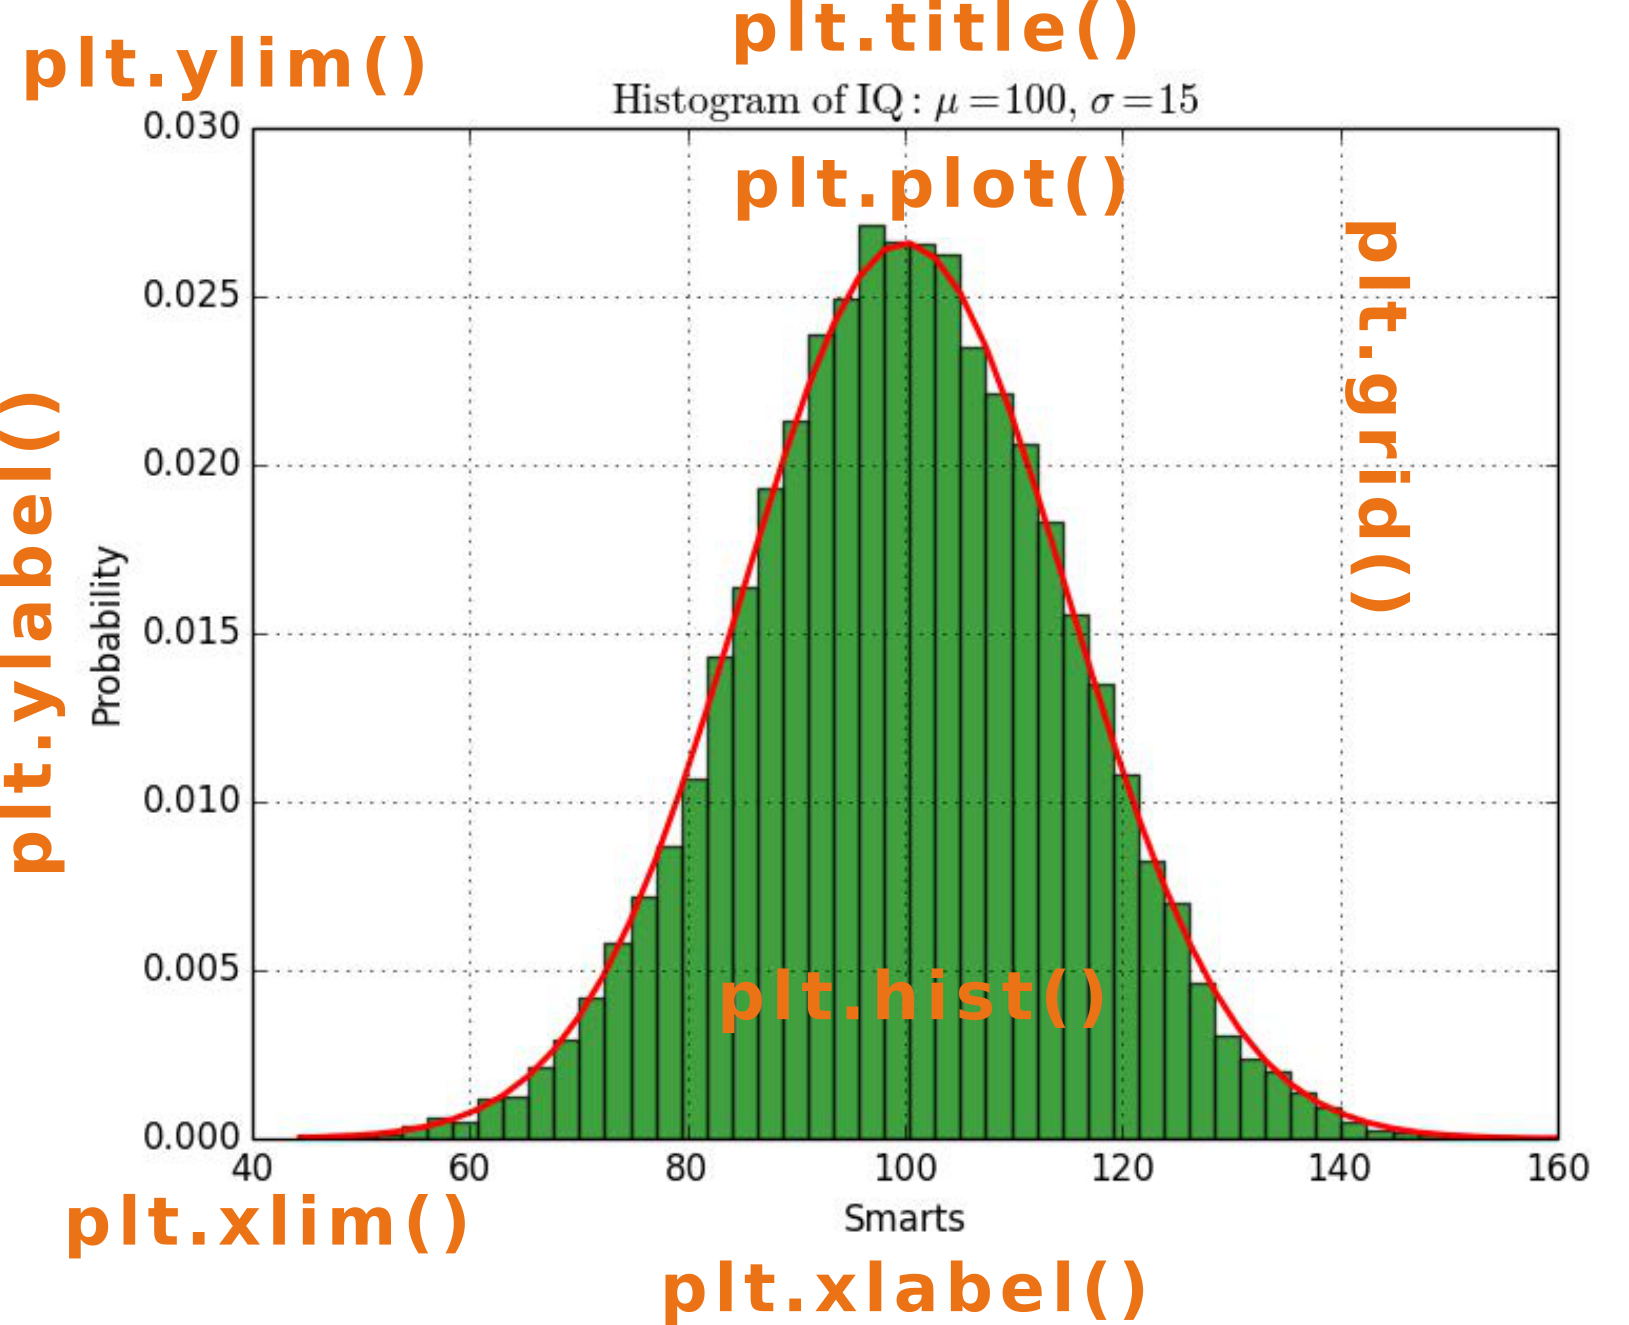
\includegraphics[width=1.\linewidth]{./histogram_labels.png}
					\column{0.45\linewidth}
						Steps to create a plot using matplotlib:\\
						{\color{sharky_main}\small 1} Import libraries\\ 
						{\color{sharky_main}\small 2} Prepare data\\
						{\color{sharky_main}\small 3} Create plot\\
						{\color{sharky_main}\small 4} Customize plot\\
						{\color{sharky_main}\small 5} Show / Save plot\\
				\end{columns}
			\end{tcolorbox}
			
			\begin{tcolorbox}[title={\small 1} Import libraries]
				%listings is used to write python code in a Beamer presentation
				\begin{lstlisting}[numbers=none]
>>> import numpy as np
>>> import matplotlib.mlab as mlab
>>> import matplotlib.pyplot as plt
				\end{lstlisting} 
			\end{tcolorbox}
			
			\begin{tcolorbox}[title={\small 2} Prepare data]
				\begin{lstlisting}[numbers=none]
>>> mu, sigma = 100, 15
>>> x = mu + sigma*np.random.randn(10000)
				\end{lstlisting} 
			\end{tcolorbox}	
		
		\column{0.5\linewidth}	
			\begin{tcolorbox}[title={\small 3} Create plot]
				\begin{lstlisting}[numbers=none]
>>> n, bins, patches = plt.hist(x, 50, normed=1, facecolor='green', alpha=0.75)
>>> y = mlab.normpdf(bins, mu sigma)
>>> l = plt.plot(bins, y 'r-', linewidth=2)
				\end{lstlisting} 
			\end{tcolorbox}
			
			\begin{tcolorbox}[title={\small 4} Customize plot]
				\begin{lstlisting}[numbers=none]
>>> plt.xlabel('Smarts')
>>> plt.ylabel('Probability')
>>> plt.title(r'$\mathrm{Histogram of IQ:} \mu=100, \sigma=15$')
>>> plt.xlim(40,160)
>>> plt.ylim(0,0.03)
>>> plt.grid(True)
				\end{lstlisting} 
			\end{tcolorbox}

			\begin{tcolorbox}[title={\small 5} Show / Save plot]
				\begin{lstlisting}[numbers=none]
>>> plt.savefi('histogram.png')
>>> plt.show()
				\end{lstlisting}
			\end{tcolorbox}
	\end{columns}
\end{frame}



\end{document}

